% Options for packages loaded elsewhere
\PassOptionsToPackage{unicode}{hyperref}
\PassOptionsToPackage{hyphens}{url}
%
\documentclass[
  ignorenonframetext,
]{beamer}
\usepackage{pgfpages}
\setbeamertemplate{caption}[numbered]
\setbeamertemplate{caption label separator}{: }
\setbeamercolor{caption name}{fg=normal text.fg}
\beamertemplatenavigationsymbolsempty
% Prevent slide breaks in the middle of a paragraph
\widowpenalties 1 10000
\raggedbottom
\setbeamertemplate{part page}{
  \centering
  \begin{beamercolorbox}[sep=16pt,center]{part title}
    \usebeamerfont{part title}\insertpart\par
  \end{beamercolorbox}
}
\setbeamertemplate{section page}{
  \centering
  \begin{beamercolorbox}[sep=12pt,center]{part title}
    \usebeamerfont{section title}\insertsection\par
  \end{beamercolorbox}
}
\setbeamertemplate{subsection page}{
  \centering
  \begin{beamercolorbox}[sep=8pt,center]{part title}
    \usebeamerfont{subsection title}\insertsubsection\par
  \end{beamercolorbox}
}
\AtBeginPart{
  \frame{\partpage}
}
\AtBeginSection{
  \ifbibliography
  \else
    \frame{\sectionpage}
  \fi
}
\AtBeginSubsection{
  \frame{\subsectionpage}
}
\usepackage{amsmath,amssymb}
\usepackage{lmodern}
\usepackage{iftex}
\ifPDFTeX
  \usepackage[T1]{fontenc}
  \usepackage[utf8]{inputenc}
  \usepackage{textcomp} % provide euro and other symbols
\else % if luatex or xetex
  \usepackage{unicode-math}
  \defaultfontfeatures{Scale=MatchLowercase}
  \defaultfontfeatures[\rmfamily]{Ligatures=TeX,Scale=1}
\fi
% Use upquote if available, for straight quotes in verbatim environments
\IfFileExists{upquote.sty}{\usepackage{upquote}}{}
\IfFileExists{microtype.sty}{% use microtype if available
  \usepackage[]{microtype}
  \UseMicrotypeSet[protrusion]{basicmath} % disable protrusion for tt fonts
}{}
\makeatletter
\@ifundefined{KOMAClassName}{% if non-KOMA class
  \IfFileExists{parskip.sty}{%
    \usepackage{parskip}
  }{% else
    \setlength{\parindent}{0pt}
    \setlength{\parskip}{6pt plus 2pt minus 1pt}}
}{% if KOMA class
  \KOMAoptions{parskip=half}}
\makeatother
\usepackage{xcolor}
\newif\ifbibliography
\usepackage{graphicx}
\makeatletter
\def\maxwidth{\ifdim\Gin@nat@width>\linewidth\linewidth\else\Gin@nat@width\fi}
\def\maxheight{\ifdim\Gin@nat@height>\textheight\textheight\else\Gin@nat@height\fi}
\makeatother
% Scale images if necessary, so that they will not overflow the page
% margins by default, and it is still possible to overwrite the defaults
% using explicit options in \includegraphics[width, height, ...]{}
\setkeys{Gin}{width=\maxwidth,height=\maxheight,keepaspectratio}
% Set default figure placement to htbp
\makeatletter
\def\fps@figure{htbp}
\makeatother
\setlength{\emergencystretch}{3em} % prevent overfull lines
\providecommand{\tightlist}{%
  \setlength{\itemsep}{0pt}\setlength{\parskip}{0pt}}
\setcounter{secnumdepth}{-\maxdimen} % remove section numbering
\ifLuaTeX
  \usepackage{selnolig}  % disable illegal ligatures
\fi
\IfFileExists{bookmark.sty}{\usepackage{bookmark}}{\usepackage{hyperref}}
\IfFileExists{xurl.sty}{\usepackage{xurl}}{} % add URL line breaks if available
\urlstyle{same} % disable monospaced font for URLs
\hypersetup{
  pdftitle={Group 11, diamonds dataset},
  pdfauthor={Tom Tribe, Ken MacIver, Jundi Yang, Mei Huang},
  hidelinks,
  pdfcreator={LaTeX via pandoc}}

\title{Group 11, diamonds dataset}
\author{Tom Tribe, Ken MacIver, Jundi Yang, Mei Huang}
\date{2022-09-15}

\begin{document}
\frame{\titlepage}

\begin{frame}{Group Members (photos)}
\protect\hypertarget{group-members-photos}{}
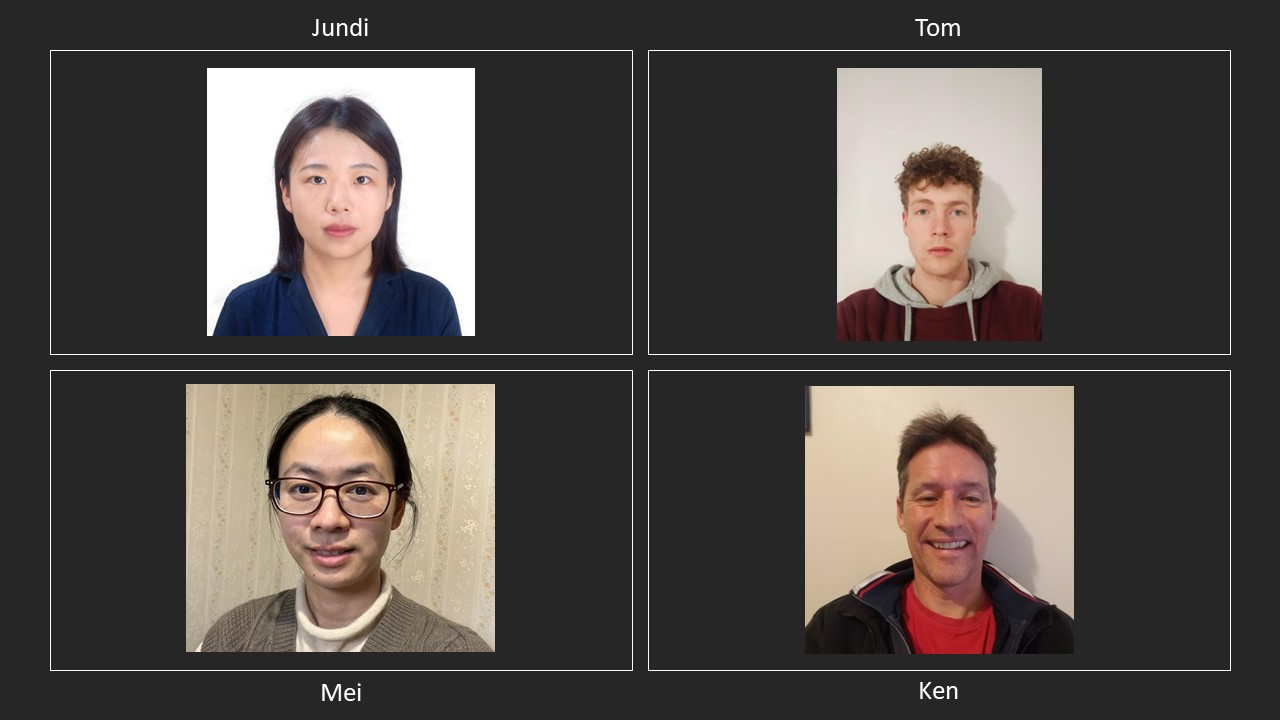
\includegraphics{./Photos3.jpg}
\end{frame}

\begin{frame}{Group Members (name, email, ORCID)}
\protect\hypertarget{group-members-name-email-orcid}{}
Tom Tribe

\begin{itemize}
\tightlist
\item
  \href{mailto:tom.tribe2016@gmail.com}{\nolinkurl{tom.tribe2016@gmail.com}}
\item
  0000-0002-5002-8066
\end{itemize}

Ken MacIver

\begin{itemize}
\tightlist
\item
  \href{mailto:ken.maciver68@gmail.com}{\nolinkurl{ken.maciver68@gmail.com}}
\item
  0000-0001-8999-4598
\end{itemize}

Jundi Yang

\begin{itemize}
\tightlist
\item
  \href{mailto:ivyli112358@gmail.com}{\nolinkurl{ivyli112358@gmail.com}}
\item
  0000-0003-0888-9564
\end{itemize}

Mei Huang

\begin{itemize}
\tightlist
\item
  \href{mailto:huangmei139@gmail.com}{\nolinkurl{huangmei139@gmail.com}}
\item
  0000-0003-2401-0679
\end{itemize}
\end{frame}

\begin{frame}{The Diamonds dataset}
\protect\hypertarget{the-diamonds-dataset}{}
\begin{itemize}
\tightlist
\item
  This large dataset has 53940 rows (diamonds) of ten variables (approx
  540,000 values)\linebreak 
\item
  Slow to process!\linebreak
\item
  Nine of the variables are various measures of diamond size and
  quality, while the tenth is the price\linebreak
\item
  We selected diamonds because it was simple to understand what each
  variable was measuring, and to have the opportunity to work with a
  large dataset\linebreak
\item
  Particularly interested in which variables are most predictive of
  diamond price
\end{itemize}
\end{frame}

\begin{frame}{The Variables}
\protect\hypertarget{the-variables}{}
\textcolor{red}{red font = categorical variable}

\begin{itemize}
\tightlist
\item
  carat: the diamond's weight
\item
  \textcolor{red}{cut: a measure of quality}
\item
  \textcolor{red}{color: a measure of colour quality}
\item
  \textcolor{red}{clarity: a measure of clearness}
\item
  x: length in mm
\item
  y: width in mm
\item
  z: depth in mm
\item
  depth: total depth percentage
\item
  table: width of top of diamond relative to widest point
\item
  price: the price of the diamond in US dollars
\end{itemize}

(List adapted from list at kaggle.com).
\end{frame}

\begin{frame}{The Response Variable}
\protect\hypertarget{the-response-variable}{}
`Price' seemed to us to be the obvious response variable.
\end{frame}

\begin{frame}[fragile]{Data Visualization (the dataset)}
\protect\hypertarget{data-visualization-the-dataset}{}
\footnotesize

\begin{verbatim}
##   carat     cut color clarity depth table price    x    y    z
## 1  0.23   Ideal     E     SI2  61.5    55   326 3.95 3.98 2.43
## 2  0.21 Premium     E     SI1  59.8    61   326 3.89 3.84 2.31
## 3  0.23    Good     E     VS1  56.9    65   327 4.05 4.07 2.31
## 4  0.29 Premium     I     VS2  62.4    58   334 4.20 4.23 2.63
## 5  0.31    Good     J     SI2  63.3    58   335 4.34 4.35 2.75
\end{verbatim}

\normalsize
\end{frame}

\begin{frame}{Data Visualisation (pairs plot)}
\protect\hypertarget{data-visualisation-pairs-plot}{}
\begin{figure}
\centering
\includegraphics{./pairs plot.jpg}
\caption{Pairs plot}
\end{figure}
\end{frame}

\begin{frame}{Other things of interest}
\protect\hypertarget{other-things-of-interest}{}
The EDA revealed the following:

\begin{itemize}
\tightlist
\item
  some variables not Normally distributed\linebreak
\item
  long right tail for `price' due to a few very expensive
  diamonds\linebreak
\item
  some zero values\linebreak
\item
  `price' probably follows a beta distribution (from the Cullen-Frey
  plot)
\end{itemize}
\end{frame}

\begin{frame}{Next Steps}
\protect\hypertarget{next-steps}{}
\begin{itemize}
\tightlist
\item
  Principal Component Analysis\linebreak
\item
  Regression using the Principal Components\linebreak
\item
  Find best predictor variable for price
\end{itemize}
\end{frame}

\end{document}
